\documentclass[conference,harvard,brazil,english]{sbatex}
\usepackage[utf8]{inputenc}
\usepackage{float}
\usepackage{ae}
\usepackage{amsfonts, amssymb}
\usepackage{amsmath}
\usepackage{graphicx}
\usepackage{indentfirst}
\usepackage{ae}
\usepackage{gensymb}
\usepackage{caption} 
\usepackage{epstopdf}
\usepackage{leading}
\usepackage[table,xcdraw]{xcolor}
\usepackage{tablefootnote}

\makeatletter
\def\verbatim@font{\normalfont\ttfamily\footnotesize}
\makeatother
\usepackage{amsmath}
% --------------------------------------------------
\begin{document}
    \title{Síntese de Controladores para um Sistema de Controle de Velocidade de um Veículo}
    \author{Thalles Oliveira Campagnani}{thallescampagnani@gmail.com}
    \author{Vinicius Fernandes Vasconcelos Barbosa}{viniciusfernandesmct@gmail.com}
    %--------------------------------
    \twocolumn[
        \maketitle
        \selectlanguage{brazil}
        \nocite{nise}
        \nocite{DB95}
        \begin{abstract}
            O presente trabalho apresenta a identificação do modelo do sistema de controle de velocidade, sintetiza dois controladores diferentes por meio de técnicas distintas da abordagem do controle clássico - no caso compensador polinomial e compensador em atraso de fase - e realiza a analise e as compara, dos critérios de desempenho do sistema de malha aberta e dos sistemas em malha fechada.
        \end{abstract}
        \keywords{Compensador Polinomial, Compensador em Atraso de Fase, Controle de Velocidade.}
        \selectlanguage{english}
        \begin{abstract}
            The present work presents the identification of the speed control system model, synthesizes two different controllers through different techniques - polynomial compensator and phase delay compensator - and performs the analysis and compares the performance criteria of the open loop system and closed-loop systems.
        \end{abstract}
        \keywords{Polynomial Compensator, Phase Delay Compensator, Speed Control.}
    ]
    \selectlanguage{brazil}
    %--------------------------------
    
    \section{Introdução}
        
        Os sistemas de controle que operam em malha aberta podem apresentar diversos problemas como a falta de precisão, dinâmica lenta, instabilidade, sucessibilidade a variação de parâmetros, etc.
        
        No escopo deste, visando controlar e obter uma resposta rápida e precisa para um controle de velocidade de um pequeno veículo, foram aplicadas diferentes abordagens desenvolvidas na disciplina de Teoria de Controle, afim de verificar sua eficiência e a compreensão das mesmas pelos discentes.
        
        As técnicas consistem inicialmente em se definir critérios de desempenho para o sistema de malha fechada desejado, logo, os polos de dinâmica dominante, e então fazer uso das técnicas de síntese de compensadores - por método polinomial e por método de atraso de fase - para que os polos de malha fechada desejados sejam obtidos ao final do processo.
    
        
    \section{Objetivos}
        
    \subsection{Objetivos Gerais}
        
        O presente trabalho tem o objetivo de 
        implementar controladores ensinados na disciplina de Teoria de Controle em uma planta física, afim de demonstrar a compreensão dos métodos e a eficácia dos mesmos aplicados dentro de um sistema real.
    
    \subsection{Objetivos Específicos}
        
        Os controladores devem ser sintetizados de forma, que em sua análise de desempenho em malha fechada, se utilize o sinal de controle em toda sua extensão, e ainda, devem ser implementados com estrutura \textit{anti-windup} (subseção \ref{sub:antiwindup}) quando possível.
    
    \section{Fundamentação Teórica}
        
        \subsection{Compensador Polinomial}
        
            Seja uma função de transferência $G(s)$ dada, e deseja-se projetar um controlador polinomial $C(s)$ que gere um sistema de malha fechada $F(s)$. 
            
            Sendo,
            
            \begin{equation}
                \label{equ:Gs}
                G(s) = \frac{B(s)}{A(s)}
            \end{equation}
            
            e,
            
            \begin{equation}
                \label{equ:Cs}
                C(s) = \frac{\beta(s)}{\alpha(s)}
            \end{equation}
            
            A função de transferência pode assumir duas formas, nesse caso existem duas abordagens possíveis, com $C(s)$ no ramo de realimentação, conhecida como controlador em série, ou no ramo de malha, com o controlador em paralelo, conforme imagem abaixo:
            
            \begin{figure}[H]
                \centering
                \includegraphics[scale=0.3]{imagens/serieparalelo.png}
                \caption{Estruturas em série e em paralelo}
                \label{fig:serieparalelo}
            \end{figure}
            
            No caso em que $C(s)$ fica no ramo de malha temos que:
            
            \begin{equation}
                \label{equ:c_ramodemalha}
                F_m(s) = \frac{ C(s) G(s) } { 1 + C(s) G(s) } = \frac { B(s) \beta(s) } { B(s) \beta(s) + A(s) \alpha(s) }
            \end{equation}
            
            No caso em que $C(s)$ fica no ramo de realimentação temos que:
            
            \begin{equation}
                \label{equ:c_ramorealimentado}
                F_r(s) = \frac{ G(s) } { 1 + C(s) G(s) } = \frac { B(s) } { B(s) \beta(s) + A(s) \alpha(s) }
            \end{equation}
            
            
        \subsubsection{Equação Diofantina}
        
            Suponhamos que desejamos obter um determinado sistema de malha fechada, $F(s)$ com determinados polos dominantes dados polo polinômio característico $D(s)$ conforme definido abaixo:
            
            \begin{equation}
                \label{equ:ND}
                F(s) = \frac{N(s)}{D(s)}
            \end{equation}
                
           Igualando as equações (3) e (5), ou (4) e (5), é possível chegar equação abaixo, conhecida como Equação Diofantina:
            
            \begin{equation}
                \label{equ:diofantina}
                D(s) =  B(s) \beta(s) + A(s) \alpha(s) 
            \end{equation}
            
            Ela consiste
            
            Falar sobre $D(s)$
            
        \subsubsection{Restrições para unicidade de solução}
        
            Seja,
            
            \begin{equation}
                \label{equ:As}
                A(s) = s^n + a_1s^{n-1} + \dots + a_{n-1}s + a_n
            \end{equation}
            
            e,
            
            \begin{equation}
                \label{equ:Bs}
                B(s) = b_0s^n + b_1s^{n-1} + \dots + b_{n-1}s + b_n
            \end{equation}
        
            e por fim, $D$, sendo um polinômio estável de grau $\delta(D(s) = 2n-1)$, 
            
            \begin{equation}
                \label{equ:Ds}
                D(s) = d_0s^{2n-1} + d_1s^{2n-2} + \dots + d_{2n-2}s + d_{2n-1}
            \end{equation}
            
            Temos como restrições para a equação Diofantina ter unicidade de soluções:
            
            \begin{itemize}
            
                \item $A(s)$ ser mônico.
                
                \item $A(s)$ e $B(s)$ serem co-primos.
                
                \item $\delta (D(s)) = 2n-1$
                
            \end{itemize}
            
            E a solução tem o formato abaixo:
            
            \begin{equation}
                \label{equ:alphas}
                \alpha(s) = \alpha_0s^{n-1} + \alpha_1s^{n-2} + \dots + \alpha_{n-2}s + \alpha_{n-1}
            \end{equation}
            
            e,
            
            \begin{equation}
                \label{equ:betas}
                \beta(s) = \beta_0s^{n-1} + \beta_1s^{n-2} + \dots + \beta_{n-2}s + \beta_{n-1}
            \end{equation}
            
            Sendo $\alpha(s)$ e $\beta(s)$ polinômios de grau $(n-1)$.
            
        \subsubsection{Solução da Equação Diofantina}
            
            Seja a matriz de Sylvester $E$ com dimensões 2n x 2n dada abaixo:
            
            \begin{equation}
                \label{mat:sylvester}
                E = 
                \begin{bmatrix}
                a_n & 0 & \dots & 0 & b_n & 0 & \dots & 0 \\
                a_{n-1} & a_n & \dots & 0 & b_{n-1} & b_n & \dots & 0 \\
                \vdots & a_{n-1} & \dots & 0 & \vdots & b_{n-1} & \dots & 0 \\
                a_1 & \vdots & \ddots & \vdots & b_1 & \vdots & \ddots & \vdots \\
                1 & a_1 & \dots & a_{n-1} & b_0 & b_1 & \dots & b_{n-1} \\
                0 & 1 & \dots & a_{n-2} & 0 & b_0 & \dots & b_{n-2} \\
                \vdots & \vdots & \ddots & \vdots & \vdots & \ddots & \dots & 0 \\
                0 & 0 & \dots & a_1 & 0 & 0 & \dots & b_1 \\
                0 & 0 & \dots & 1 & 0 & 0 & \dots & b_0
                \end{bmatrix}
            \end{equation}
            
            Seja a matriz M abaixo:
            
            \begin{equation}
                M = \begin{bmatrix}
                \alpha_{n-1} \\ \alpha_{n-2} \\ \vdots \\ \alpha_{0} \\ \beta_{n-1} \\ \beta_{n-2} \\ \vdots \\ \beta_{0}
                \end{bmatrix}
            \end{equation}
            
            Seja a matriz $D$ abaixo, definida pelo polinômio $D(s)$, contendo os termos do polinômio cujas raízes representam os polos de malha fechados desejados:
            
            \begin{equation}
            \label{mat:D}
                D = \begin{bmatrix}
                d_{2n-1} \\ d_{2n-2} \\ \vdots \\ d_1 \\ d_0
                \end{bmatrix}
            \end{equation}
        
            Assim a solução é dada por:
            
            \begin{equation}
                M = E^{-1}D
            \end{equation}
            
        \subsubsection{Pré-compensação da Malha Fechada}
            
            Como o presente método não aloca polo na origem, não garante erro de regime permanente nulo para entradas degrau para sistemas de tipo 0, neste caso faz-se a necessidade de pré-compensar a malha fechada para garantir ganho unitário.
            
            O ganho de malha fechada é dado por:
            
            \begin{equation}
                G_{mf} = \frac{1}{1 + K_p}
            \end{equation}
            
            Para torná-lo unitário é necessário pré-compensar a malha fechada com o inverso do ganho atual.
            
            Logo temos que o pré-compensador $p$ é:
            
            \begin{equation}
            \label{equ:precompensador}
             p = \frac{n}{s+n}
            \end{equation}
            
            Além disso, como os critérios de desempenho estabelecidos através do polinômio característico $D(s)$ partem do pré-suposto que $\delta(N(s))=1$, e é sabido que $\delta(N(s))>1$ para $\delta(G(s))>1$, faz a necessidade, neste caso, de pré-compensar os zeros de malha fechada, porém tal compensação apenas é possível quando  $N(s)=1$ é estável, ou seja, $F(s)$ não possui zeros de fase não miníma.
            
            Seja $P(s)$ a função de transferência do pré-compensador dada pela equação abaixo:
            
            \begin{equation}
                P(s) = \frac{1}{B(s) \beta(s)}
            \end{equation}
            
            E seja $E(s)$ a função de transferência da malha fechada pré-compensada, temos que:
            
            \begin{equation}
                E(s) = P(s)F(s) =  \frac { 1 } { D(s) }
            \end{equation}
            
        
        \subsection{Compensador em Atraso}
            \label{sub:compensadoratraso}
            
            O método de compensação em atraso ou avanço de fase consiste em definir polos de malha fechada a partir de suas características desejadas de desempenho.
            Polos estes que são alocados através da colocação de um zero e um polo no sistema, que a depender de sua ordenação geram um atraso ou um avanço na fase.
            
            \subsubsection{Cálculo de Polos Através de Parâmetros de Desempenho}
            
                Definidos parâmetros de desempenho desejados para o sistema, é possível se obter o par de polos que em malha fechada retornam a dinâmica definida.
                Essa definição pode ser feita de forma simplificada a partir dos valores de $\zeta$ (ou o percentual de sobressinal) e $t_s$, assim como outros parâmetros. Com estes dois, já se obtém o valor de $\omega_n$.
                
                O primeiro par de polos é definido por:
                \begin{equation}
                    \label{equ:polos12}
                    P_{1,2} = -\zeta \omega_n \pm \sqrt{\zeta^2-1}
                \end{equation}
                
                O polo pode ser definido de forma conveniente, neste caso sendo definido em $0$ para adicionar um integrador. Sabendo que a soma dos ângulos resulta em $-180\degree$, e que os zeros e polos no têm contribuições positiva e negativa, respectivamente:
                
                \begin{equation}
                    \label{equ:contribuicaoangular}
                    - \phi + 90\degree \pm \beta_1 \pm \beta_2 = -180\degree
                \end{equation}
                
                Tendo que $\beta_1$ e $\beta_2$ são as contribuições angulares relativos dos polos e zeros relativos ao par de polos complexos definidos.
                
                Obtido o valor de $\phi$, o zero estará alocado em:
                
                \begin{equation}
                    \label{equ:polo}
                    Z_c = \frac{Re(Im(P_{1,2}))}{tan(\phi)} + \mid P \mid
                \end{equation}
            
            Sendo $P$ o valor do polo definido.
            
            \subsection{Estrutura anti-windup}
                \label{sub:antiwindup}
                Segundo \cite{silva_2000}, o anti-windup é a estrutura que "descarrega" o integrador quando o atuador entra na zona de saturação. Existem diversos métodos para a realização, mas para o escopo deste foi utilizado o método de \texttt{back-calculation}.
                
                O método de \texttt{back-calculation} consiste em re-calcular o termo integral quando o atuador atinge a saturação, de forma que o mesmo permaneça no valor limite do atuador.
        
    \section{Desenvolvimento}
    
        \subsection{Descrição da Planta }
        
            A planta consiste basicamente em um veículo de duas rodas com um atuador em cada. A primeira delas, atua na velocidade do modelo, que é a variável a ser controlada, enquanto o outro, via protocolo \textit{Bluetooth} controla o ângulo da roda dianteira, para que, atualmente, possa ser corrigido manualmente o raio de curvatura e, futuramente, implementar novas malhas de controles.
            
            São alimentadas por uma bateria de 30V, uma ponte-H com chip \texttt{LN-298} e um microcontrolador \textit{Arduino NANO}. O responsável por retornar a variação angular é um encoder \texttt{OPB-991T51}, que o sinal do mesmo é derivado em relação ao tempo para encontrar a velocidade angular e por fim ser convertida em velocidade linear, a qual é a variável a ser controlada.
            
            \subsubsection{Faixa de valores de entrada e saída}
            
                \begin{table}[H]
                    \begin{tabular}{|
                        >{\columncolor[HTML]{C0C0C0}}l |c|c|c|}
                        \hline
                        \textbf{}                                                         & \cellcolor[HTML]{C0C0C0}\textbf{PWM} & \cellcolor[HTML]{C0C0C0}\textbf{\begin{tabular}[c]{@{}c@{}}Tensão \end{tabular}} & \cellcolor[HTML]{C0C0C0}\textbf{\begin{tabular}[c]{@{}c@{}}Velocidade\end{tabular}} \\ \hline
                        
                        \textbf{\begin{tabular}[c]{@{}l@{}}Mínimo \\ (Real)\end{tabular}} & 0                                    & 0 V                                                                                      & 0 m/s                                                                                           \\ \hline
                        \textbf{\begin{tabular}[c]{@{}l@{}}P. O. \\ (Real)\tablefootnote{Ponto de Operação Real}\end{tabular}}  & 104                                  & 12 V                                                                                    & 1 m/s                                                                                         \\ \hline
                        \textbf{\begin{tabular}[c]{@{}l@{}}Máximo \\ (Real)\end{tabular}} & 170                                  & 20 V                                                                                     & 1.75 m/s                                                                                             \\ \hline
                         
                        \textbf{\begin{tabular}[c]{@{}l@{}}Mínimo \\ (\%)\end{tabular}}   & 0\%                                    & 0\%                                                                                      & 0\%                                                                                             \\ \hline
                        \textbf{\begin{tabular}[c]{@{}l@{}}P. O. \\ (\%)\tablefootnote{Ponto de Operação Percentual}\end{tabular}}    & 41,18\%                              & 41,18\%                                                                                   & 47.69\%                                                                                              \\ \hline
                        \textbf{\begin{tabular}[c]{@{}l@{}}Máximo\\ (\%)\end{tabular}}    & 100\%                                  & 100\%                                                                                    & 100\%                                                                                             \\ \hline
                       
                        
                    \end{tabular}
                \end{table}

            %Função que converte tensao para PWM
            \subsubsection{Identificação da Planta}
            
                Uma maneira de obter modelos lineares de sistemas em torno do ponto de operação, é aplicado um sinal na entrada da mesma, como por exemplo com formato de uma sinc em torno do ponto de operação - a vantagem do sinal sinc é estimular todas as frequências da planta -, e medida a variação na saída. Conforme imagem abaixo:

                \begin{figure}[H]
                    \centering
                    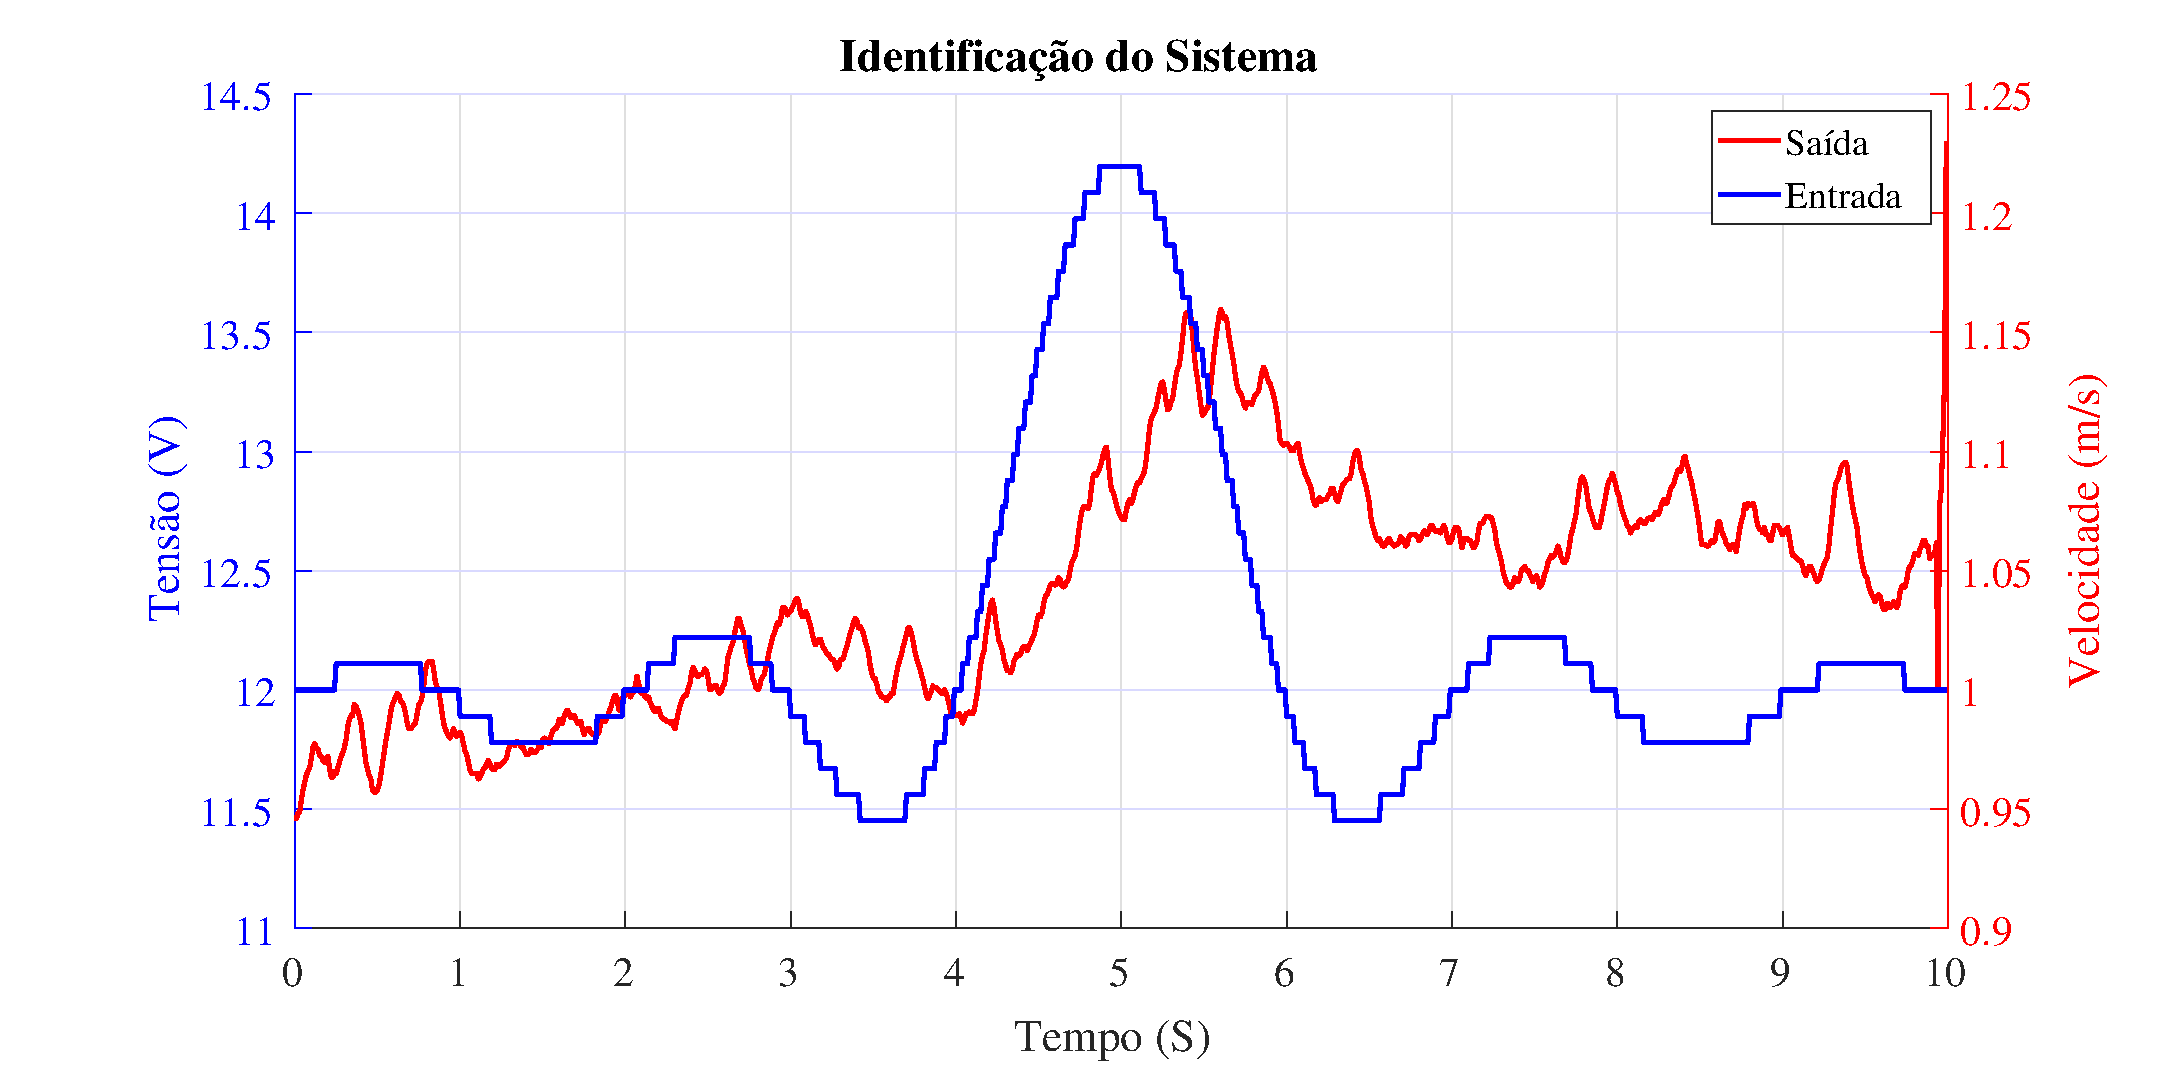
\includegraphics[width=0.5\textwidth]{imagens/identValidSat/identificacaoDoSistema.eps}
                    \caption{Identificação da planta}
                    \label{cont_poli_sc}
                \end{figure}
                
                Então o sinal de entrada e saída podem ser comparados através das ferramentas adequadas, como por exemplo através da função de identificação de sistemas do \textit{MATLAB}, \textit{ident}.
                
                Realizando este procedimento na planta em questão, é possível obter o seguinte modelo:
            
                \begin{equation}
                    \label{equ:modelo}
                    T_f(s) = \frac{0.065}{s + 0.2}
                \end{equation}
                
            \subsubsection{Validação do Modelo}
                
                É necessário verificar se o modelo identificado realmente representa a dinâmica da planta, para tal, é aplicado um outro sinal ao mesmo tempo na planta e no modelo, e comparado as saída de ambos.
                
                O sinal aplicado foi degraus com amplitudes de $\pm10\%$ em relação ao ponto de operação. O resultado pode ser conferido na imagem abaixo:
                
                \begin{figure}[H]
                    \centering
                    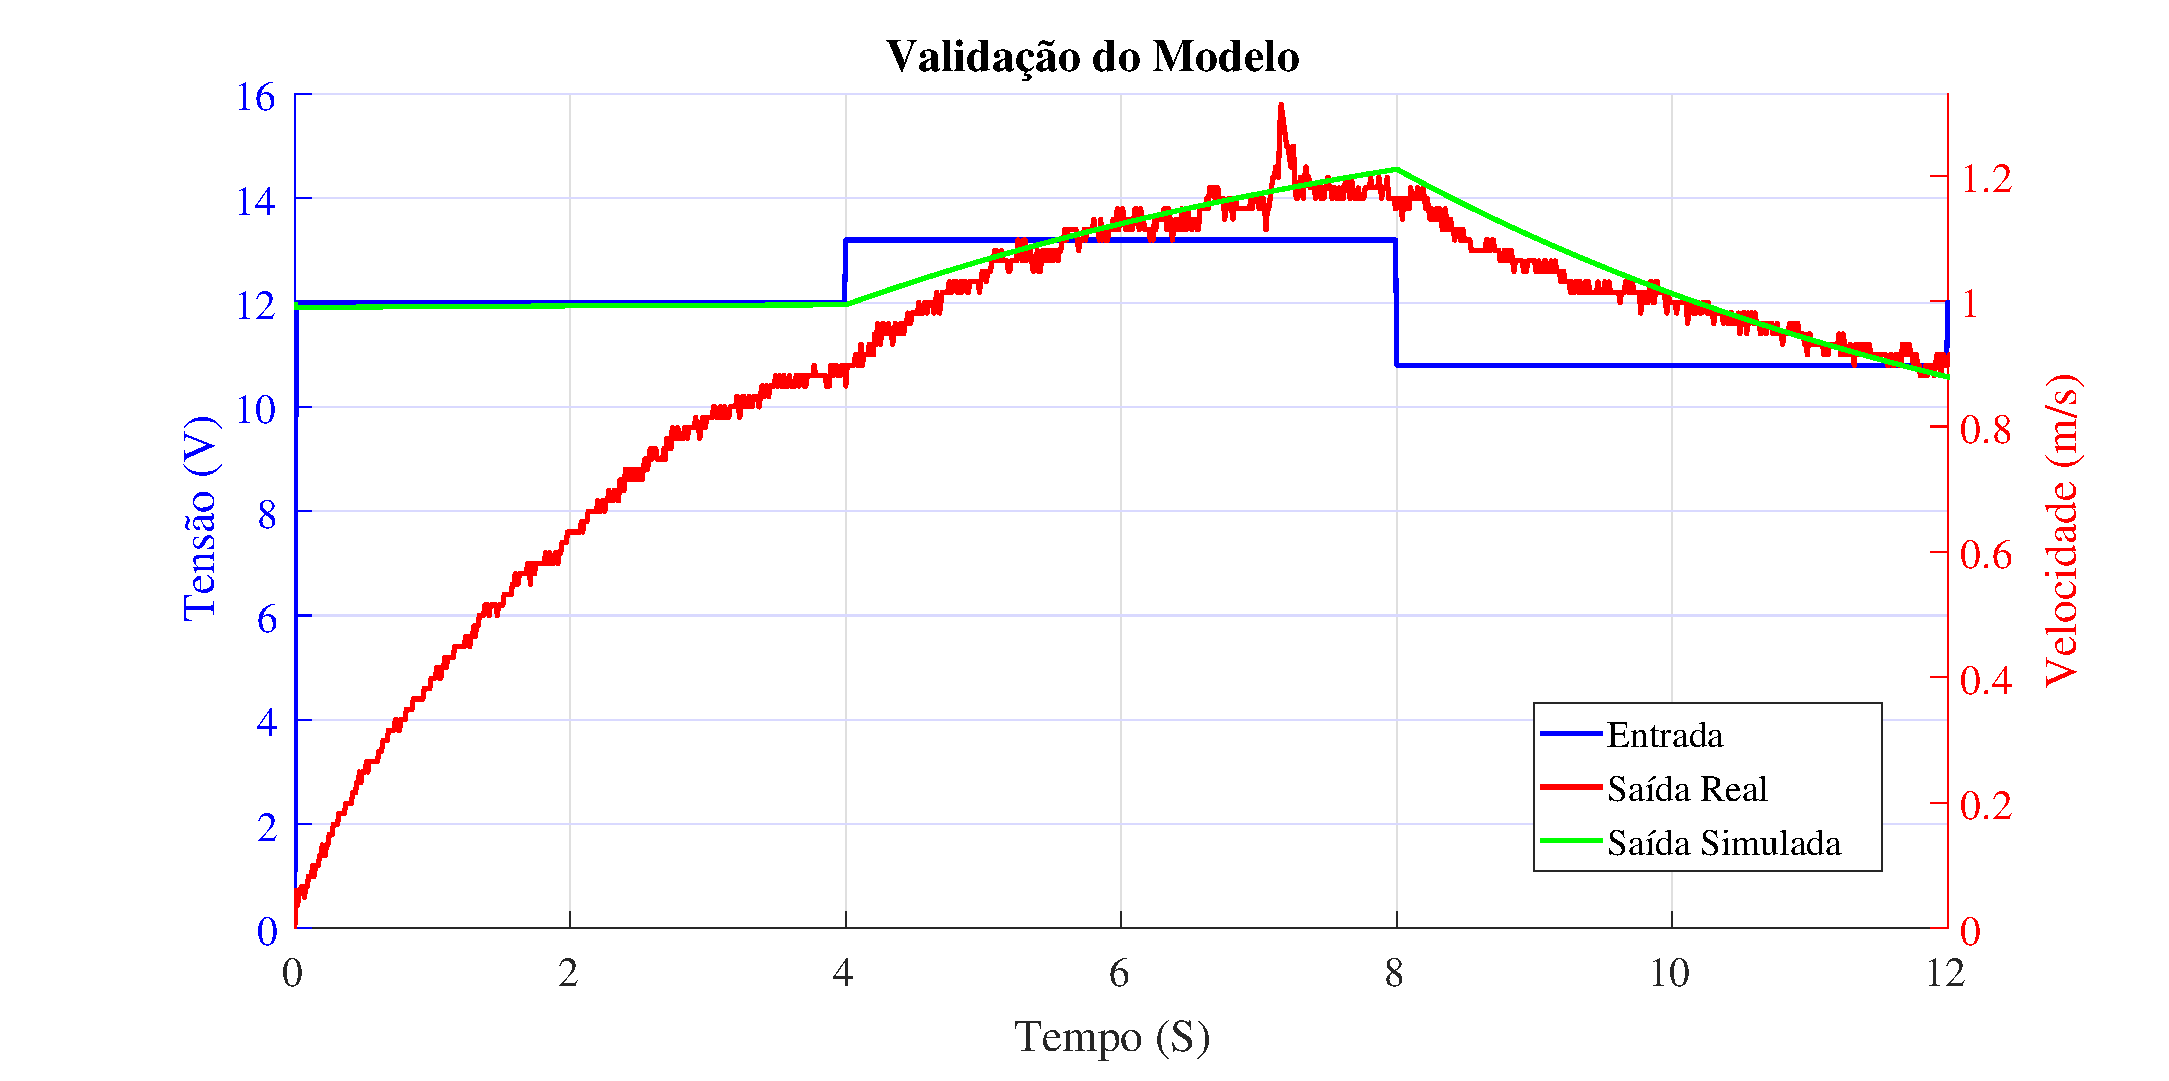
\includegraphics[width=0.5\textwidth]{imagens/identValidSat/validacaoDoModelo.eps}
                    \caption{Validação do modelo}
                    \label{fig:validacao}
                \end{figure}
                
                Como pode ser observado a saída do modelo corresponde bem a saída real da planta, logo este modelo representa bem a dinâmica da planta e o mesmo será utilizado para a síntese dos controladores.
    
            \subsubsection{Identificação da dinâmica de saturação}
                
                Identificar a dinâmica do sistema em torno do ponto de operação com o atuador saturado é importante para identificar qual os critérios de desempenho limite é possível atingir em malha fechada.
                
                Para realizar essa identificação, sendo $u$ o valor da entrada da planta, foi aplicado o $u$ de equilíbrio do ponto de operação, logo em seguida foi aplicado o $u$ de saturação, $20$ volts, e por fim um $u$ de equilíbrio de uma variação de $10\%$ do ponto de operação.
                
                \begin{figure}[H]
                    \centering
                    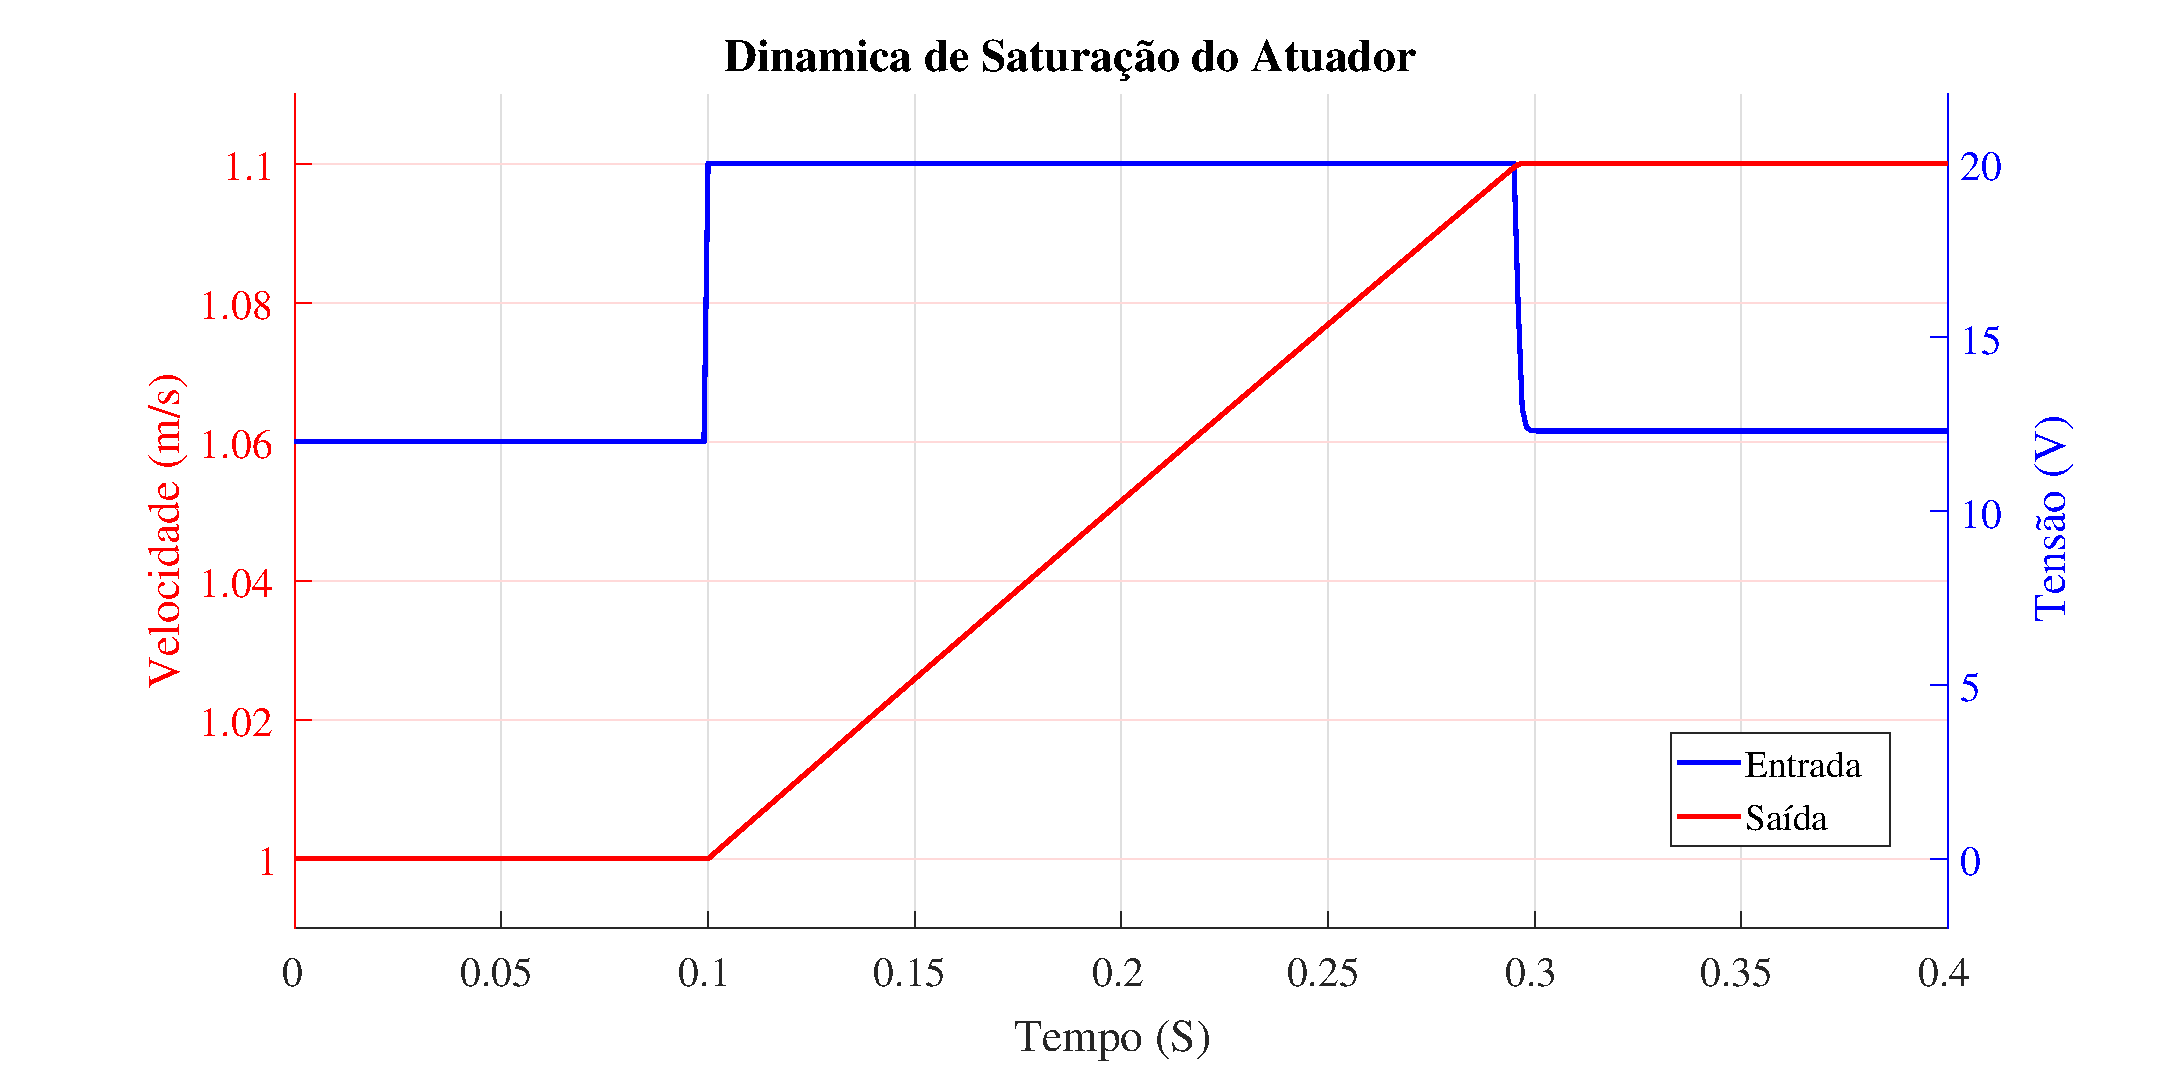
\includegraphics[width=0.5\textwidth]{imagens/identValidSat/dinamicaSaturacaoAtuador.eps}
                    \caption{Dinâmica da planta em torno do ponto de operação, com atuador saturado}
                    \label{fig:dinamicasaturada}
                \end{figure}
                
                Como pode ser observado na figura, a planta demora $200ms$ para variar $10\%$ do ponto de operação. Então só é possível especificar até no mínimo $200ms$ o tempo de acomodação para para os polos dominantes de malha fechada, ou seja, polos com frequência real de $20rad/s$
            
                
        \subsection{Critérios de Desempenho Desejados}
        
            É necessário que o sistema em malha fechada tenha o menor tempo de acomodação possível, sobressinal menor que $2\%$ e capacidade de rejeitar pertubações, devido que, outros processos dependem que a saída deste não esteja fora de uma variação percentual de $\pm 2\%$ da referência.
            
            O menor tempo de acomodação possível de ser praticado é $0.2$ segundos devido a presença da saturação do atuador, como visto na subseção anterior. Como se deseja obter o menor tempo de acomodação possível, a parte real dos polos de malha fechada serão $-20 rad/s$. A parte imaginária dos polos é calculada com base em um sobressinal de $1\%$ afim de deixar uma folga para eventuais perturbações, evitando assim extrapolar a variação máxima desejada. Realizando os cálculos é possível chegar que a parte complexa que tem esse sobressinal é $13.6438i$. Portanto:
            
            \begin{equation}
                p_{1,2} = 20 \pm 13.6438i
            \end{equation}
        
        \subsection{Compensador Polinomial e Pré-compensação}
        
        A partir dos cálculos, o polo de malha fechada deve estar localizado em $P_1 = -20$.
        
        A partir do modelo em $ \left( \ref{equ:modelo} \right)$, a matriz $E$ será:
        
        \begin{equation}
        \label{equ:matrizE}
        E= \begin{bmatrix}
        0.02 & 0.065 \\
        1 & 0 \\
        \end{bmatrix}
        \end{equation}
    
        E a matriz $D$:

        \begin{equation}
        \label{equ:matrizD}
        D = \begin{bmatrix}
        20 \\ 0
        \end{bmatrix}
        \end{equation}
        
        Tendo que $M = E^{-1}D$,
        $$
            M = \begin{bmatrix}
            0 & 1 \\ 65.3595 & -35.7843
            \end{bmatrix}
            \begin{bmatrix}
            20 \\ 0
            \end{bmatrix}
        $$
        
        Então,
        
        \begin{equation}
            \label{equ:matrizM}
            M = \begin{bmatrix}
            0 \\ 307.6923
            \end{bmatrix}
        \end{equation}
        
        E o controlador será definido por:
        
        \begin{equation}
            \label{tf:controlador}
            C(s) = 307.6923
        \end{equation}
        
        Que representa um ganho estático.
        
        \subsection{Compensador em Atraso com Estrutura Anti-windup e Pré-compensação}
        
            Com os polos de malha fechada definidos em $P_{1,2} = -20 \pm 13.6438i$, calcula-se a contribuição angular dos polos e zeros existentes no sistema afim de definir a posição do polo a ser inserido.
            
            Contribuição do pólo alocado em $0$ (integrador):
            \begin{equation}
                \label{res:beta1}
                \beta_1 = 180 - tan^{-1} \left(\frac{13.6438}{20}\right) = 145.6986\degree
            \end{equation}
            
            Contribuição do pólo alocado em $0.2$:
            \begin{equation}
                \label{res:beta1}
                \beta_2 = 180 - tan^{-1} \left(\frac{13.6438}{19.8}\right) = 145.43\degree
            \end{equation}
            
            \begin{equation}
             \phi - 145.6986\degree - 145.43\degree = -180\degree 
            \end{equation}
            
            \begin{equation}
            \label{res:phi}
            \phi = 111.1286\degree    
            \end{equation}
            
            Obtido o valor de $\phi$, a posição do zero será definida pela equação \ref{equ:polo}:
            
            \begin{equation}
                \label{res:poloatraso}
                Z_c = \left(\frac{13.6438}{tan(111.1286\degree)}\right) + 20 = 14.7275
            \end{equation}
            
            Então o controlador será dado por
            
            \begin{equation}
                \label{equ:controladorematraso}
                C_{atraso} = 612.88 \left(\frac{s + 14.7275}{s}\right)
            \end{equation}
    
    \section{Resultados e Discussões}
    
        \subsection{Sistema em Malha Aberta}
        
        O sistema em malha aberta é mostrado na figura \ref{fig:validacao}. É possível notar resposta do sistema, sem seguir a referência e de acomodação lenta, diferente das respostas em malha fechada que serão mostradas nas seções seguintes.
    
        \subsection{Sistema de malha fechada com Compensador Polinomial e pré-compensação}
        
            \begin{figure}[H]
                \centering
                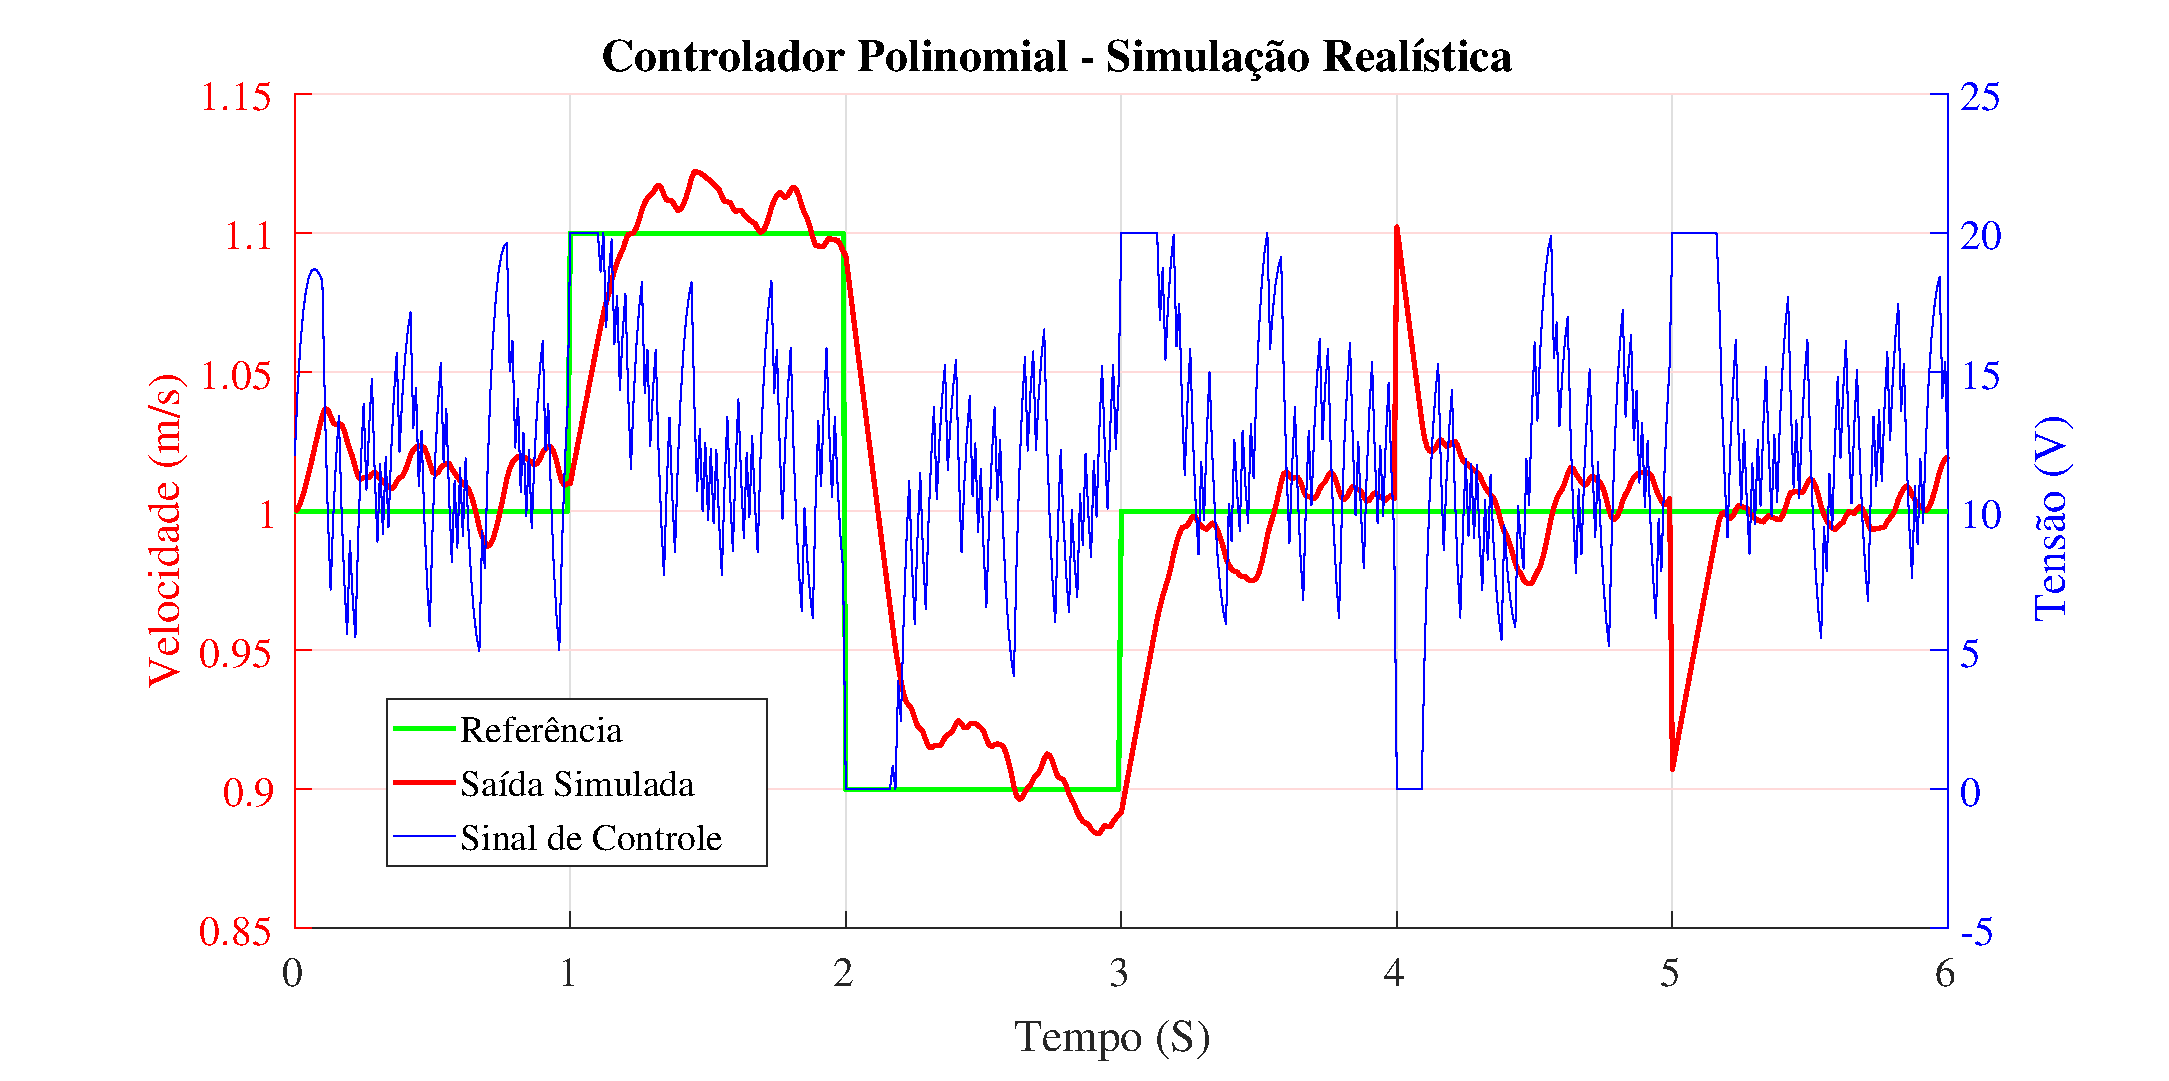
\includegraphics[width=0.5\textwidth]{imagens/polinomial/simulacaoRealisticaPolinomial.eps}
                \caption{Simulação realística com controlador desenvolvido por método polinomial.}
                \label{fig:cont_poli_simu}
            \end{figure}
            
            A simulação realística foi realizada com um sinal PRBS\footnote{Pseudo-Random Binary Signal - Sinal Binário Pseudo-Aleatório}, afim de se verificar se o controlador funciona em condições similares as reais, sem a necessidade de sair para testes em campo.
            Na figura \ref{fig:cont_poli_simu}, é possível ver que a dinâmica do sistema em malha fechada está de acordo com os parâmetros de desempenho definidos.
            
            \begin{figure}[H]
                \centering
                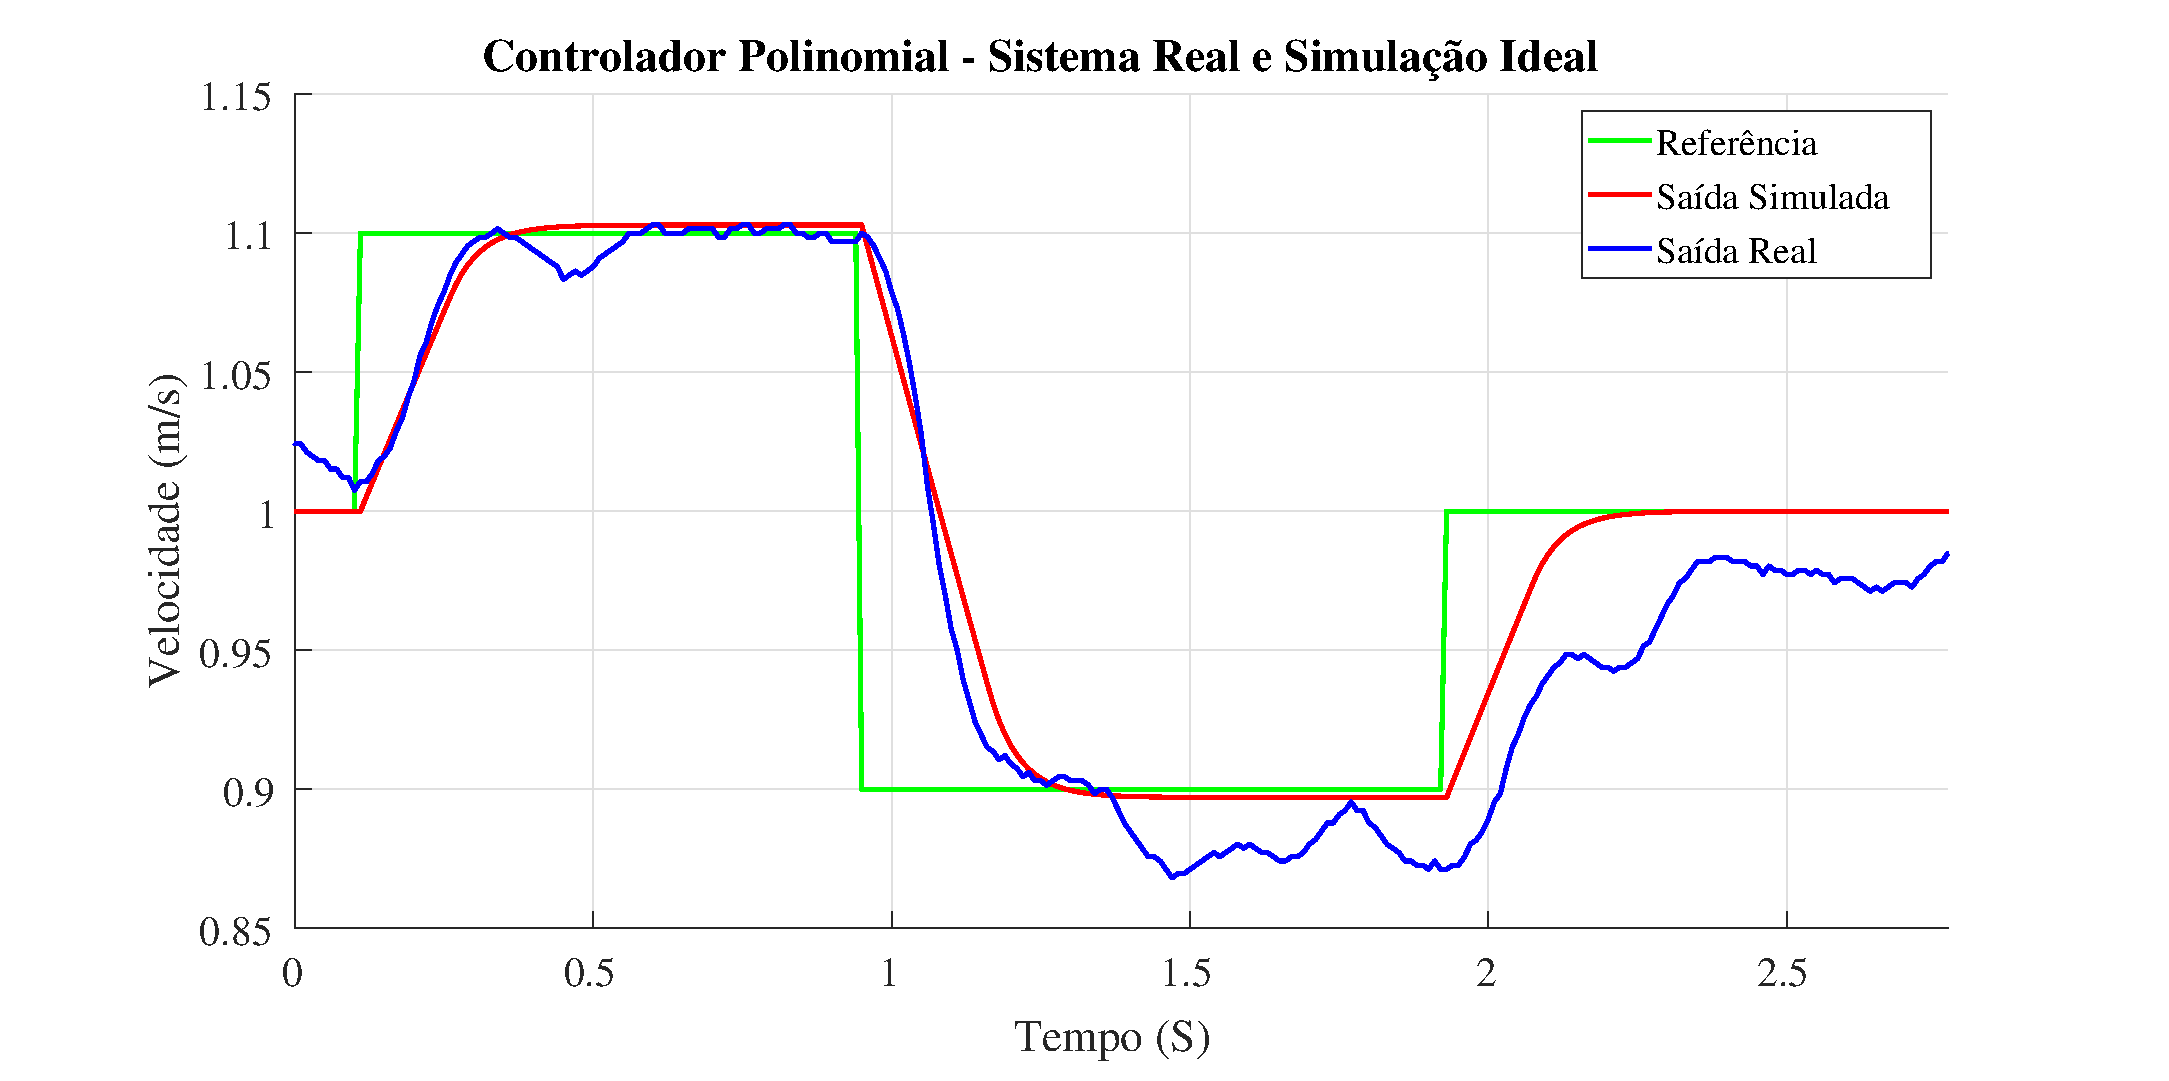
\includegraphics[width=0.5\textwidth]{imagens/polinomial/comparacaoPolinomial.eps}
                \caption{Comparação entre saída do sistema real e e saída do sistema ideal, com controlador polinomial.}
                \label{fig:cont_poli_sc}
            \end{figure}
            
            O sistema real na figura \ref{fig:cont_poli_sc} com o controlador apresentou resposta bastante similar em suas dinâmicas de subida em comparação com o modelo simulado, com variações devido as perturbações.
            
            \begin{figure}[H]
                \centering
                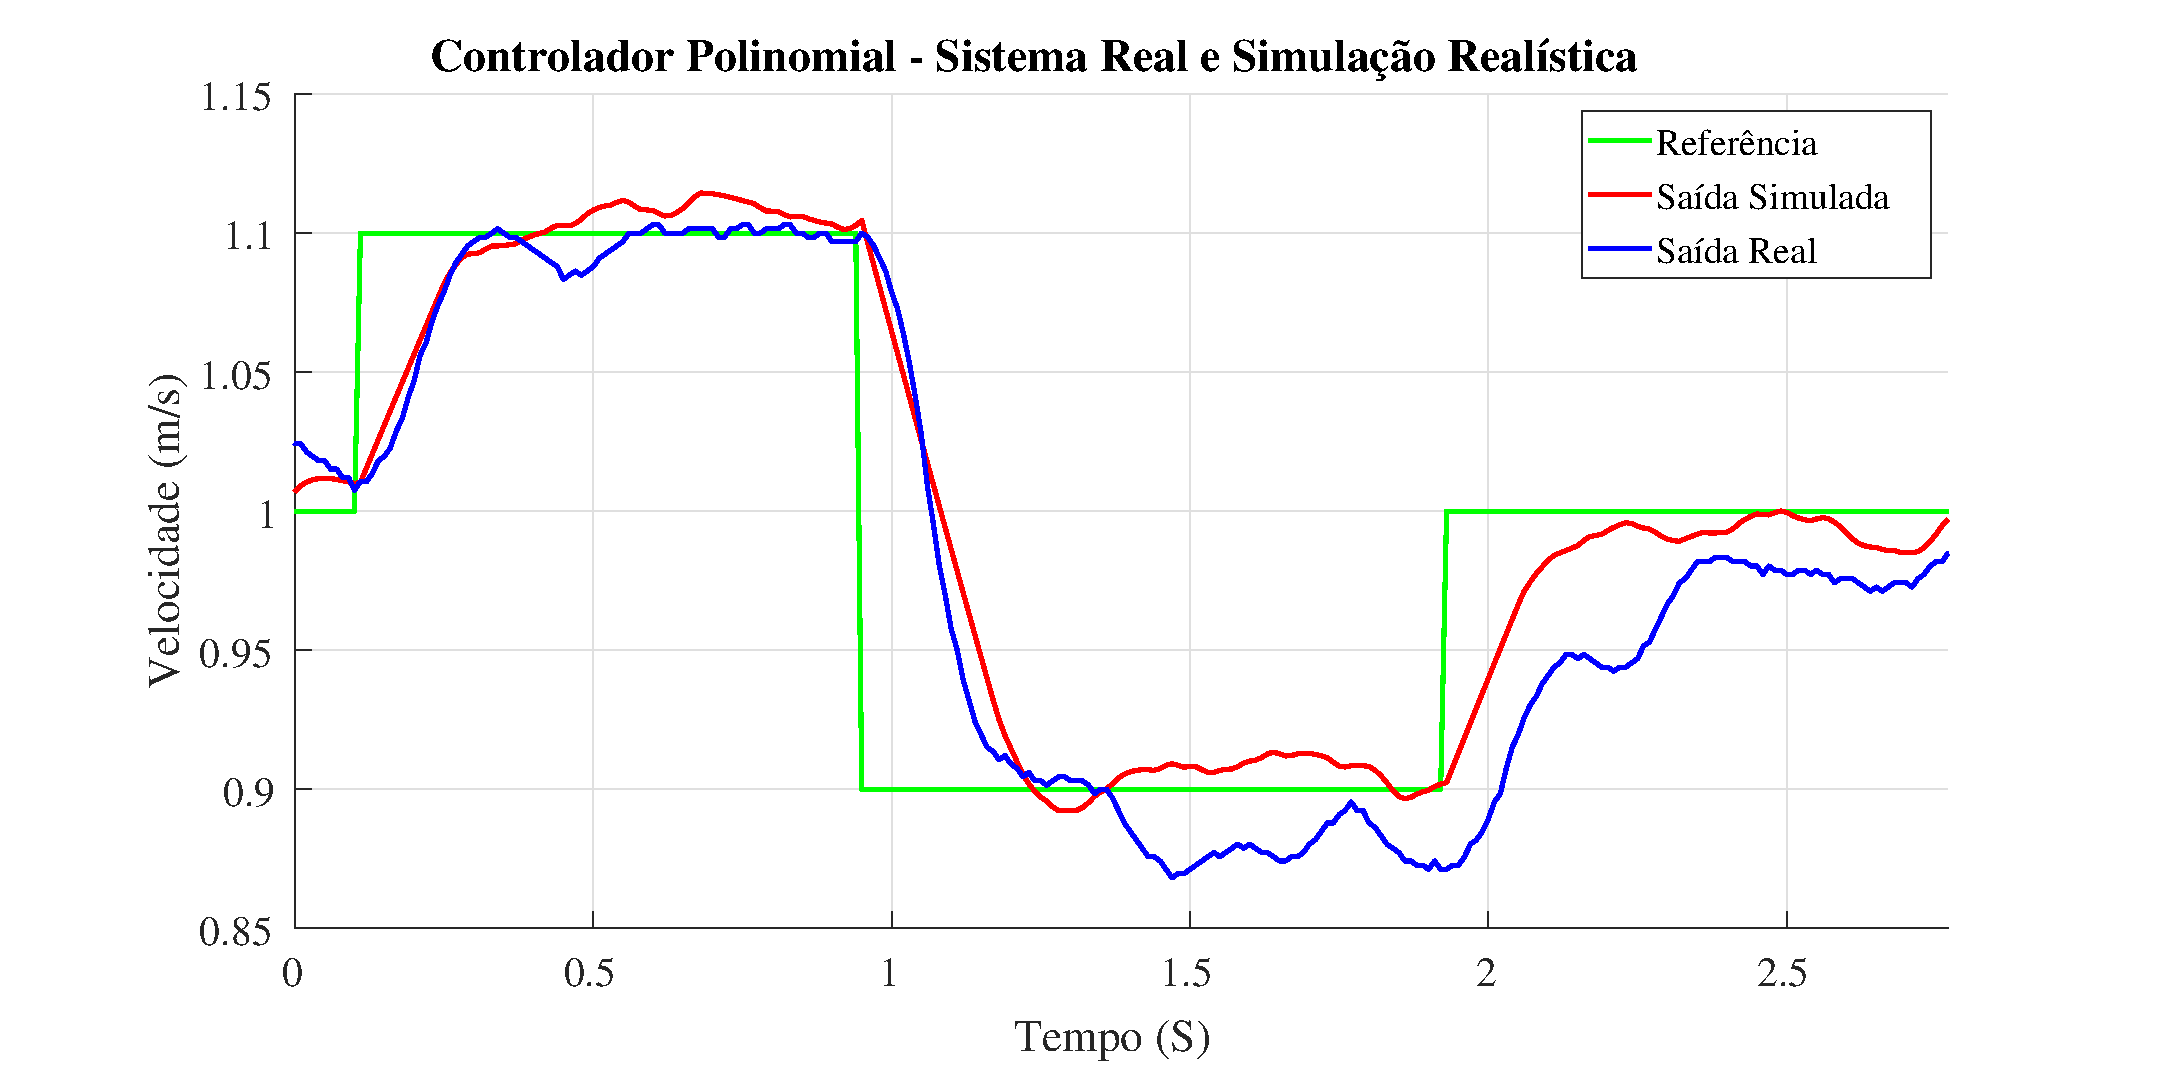
\includegraphics[width=0.5\textwidth]{imagens/polinomial/comparacaoRealisticaPolinomial.eps}
                \caption{Comparação entre a resposta do sistema realística com controlador polinomial.}
                \label{fig:realistica_poli}
            \end{figure}
            
            Na figura \ref{fig:realistica_poli}, a saída real é comparada com uma simulação realística, tendo a dinâmica ainda mais similar que a anterior, atendendo os padrões de desempenho.
        
        \subsection{Sistema de malha fechada com Compensador em Atraso com estrutura anti-windup e pré-compensação}
        
            \begin{figure}[H]
                \centering
                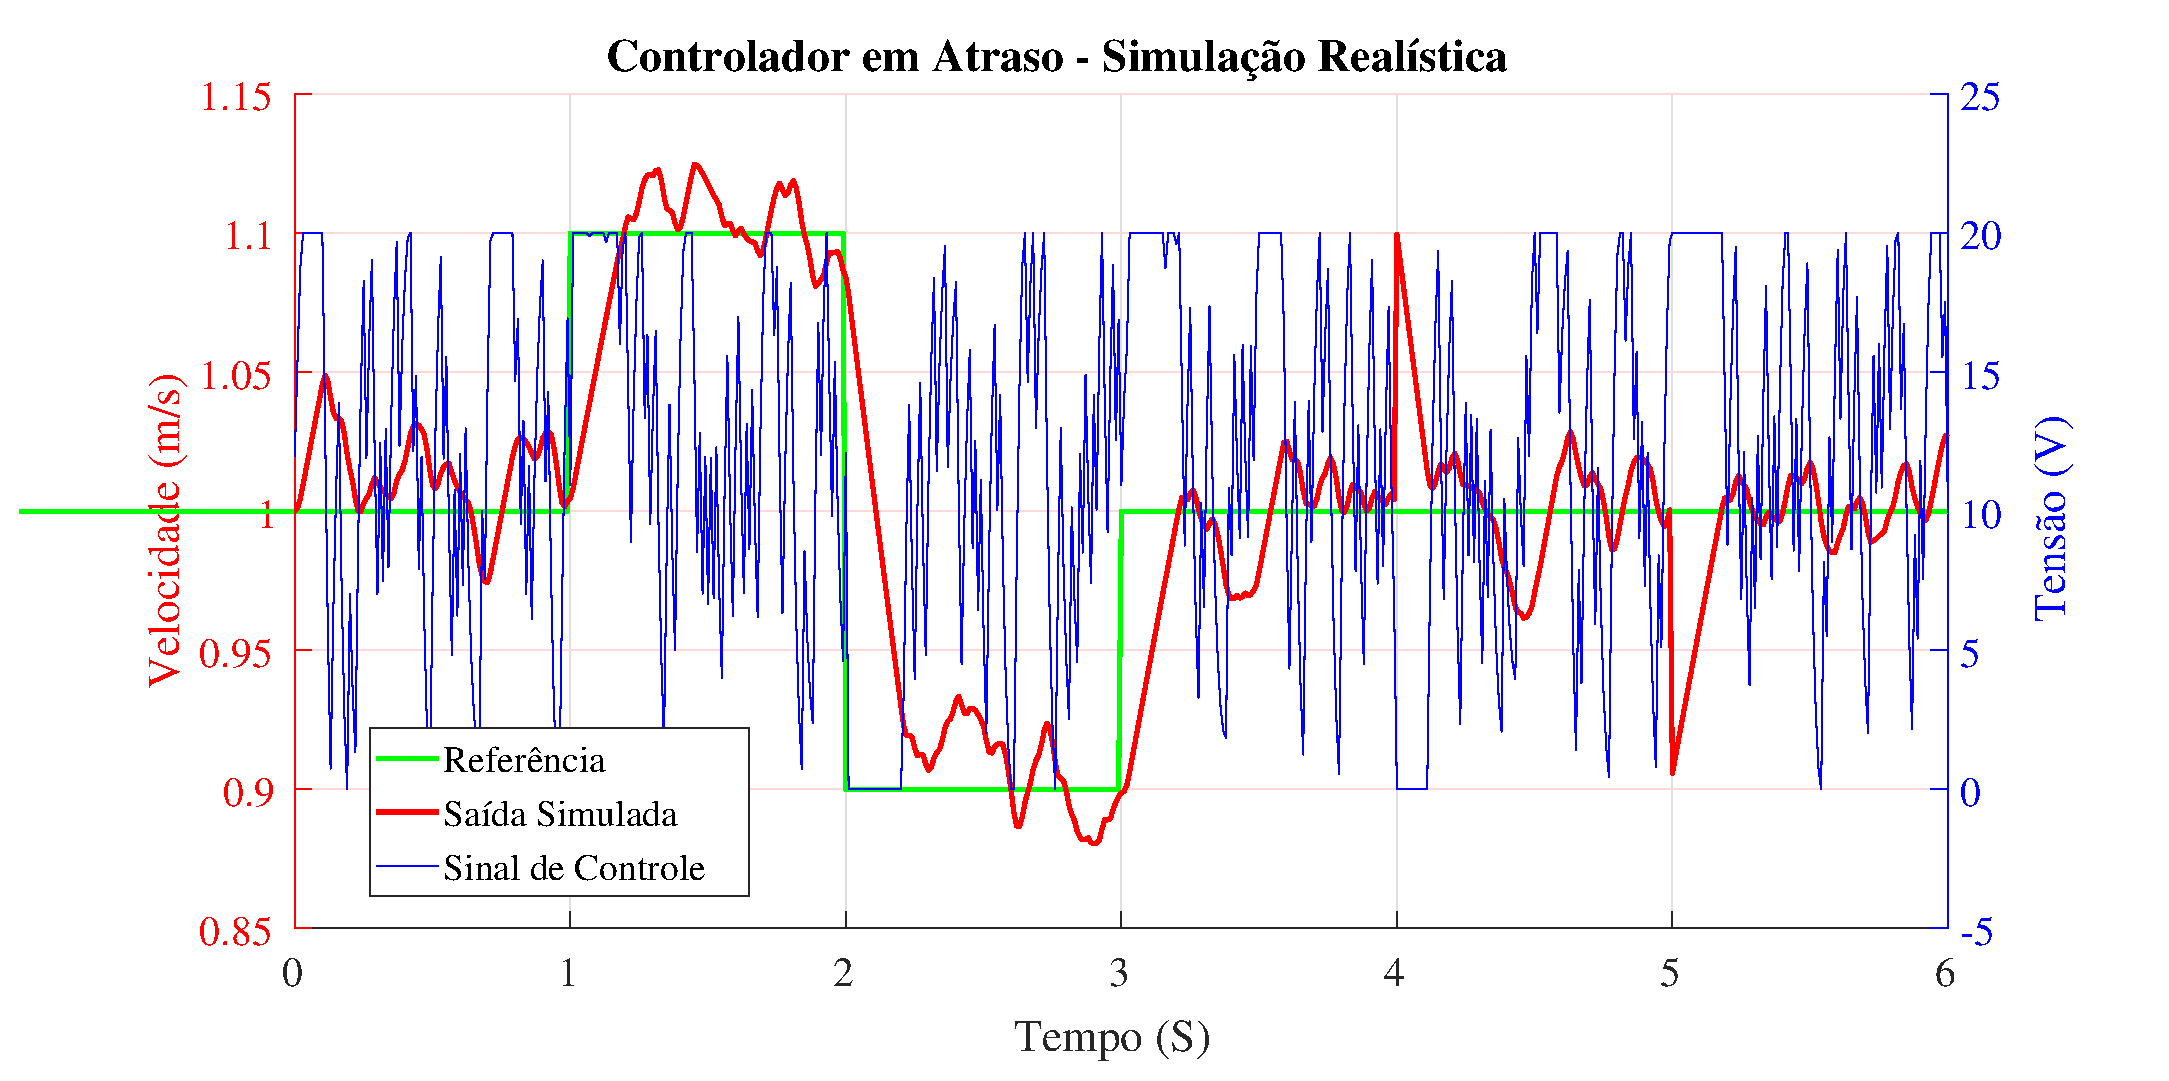
\includegraphics[width=0.5\textwidth]{imagens/atraso/simulacaoRealisticaAtraso.eps}
                \caption{Simulação realística com controlador desenvolvido por método em atraso de fase.}
                \label{fig:cont_atraso_simu}
            \end{figure}
            
            A figura \ref{fig:cont_atraso_simu} mostra o funcionamento do controlador numa simulação realística para o controlador em atraso desenvolvido, apresentando desempenho condizente com os parâmetros definidos.
            
            \begin{figure}[H]
                \centering
                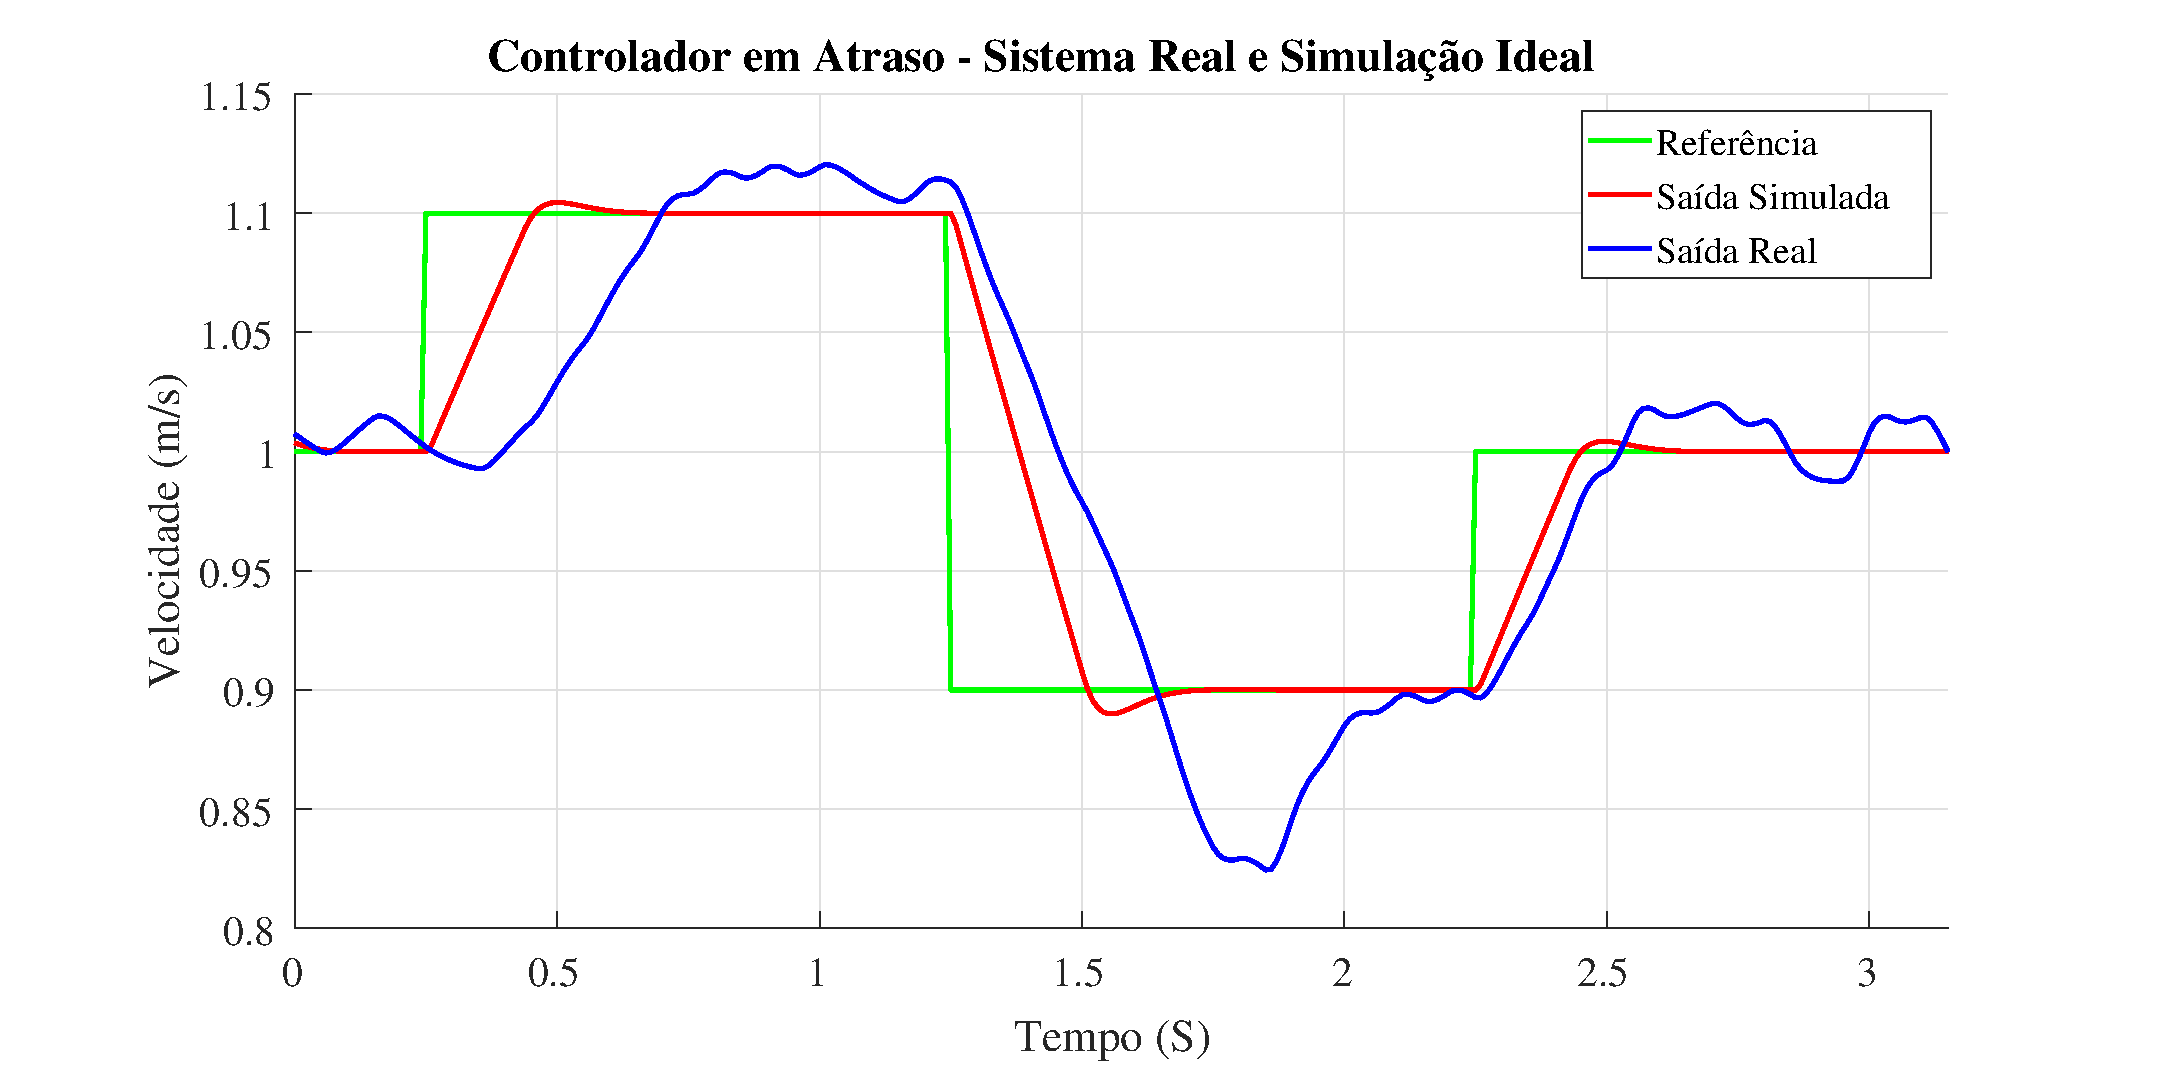
\includegraphics[width=0.5\textwidth]{imagens/atraso/compRealIdeal.eps}
                \caption{Comparação entre saída do sistema real e e saída do sistema ideal, com controlador em atraso de fase.}
                \label{fig:cont_atraso}
            \end{figure}
            
            Em \ref{fig:cont_atraso}, é possível perceber a similaridade nas respostas, com certo atraso no início mas com a dinâmica similar a esperada através do modelo.
            
            \begin{figure}[H]
                \centering
                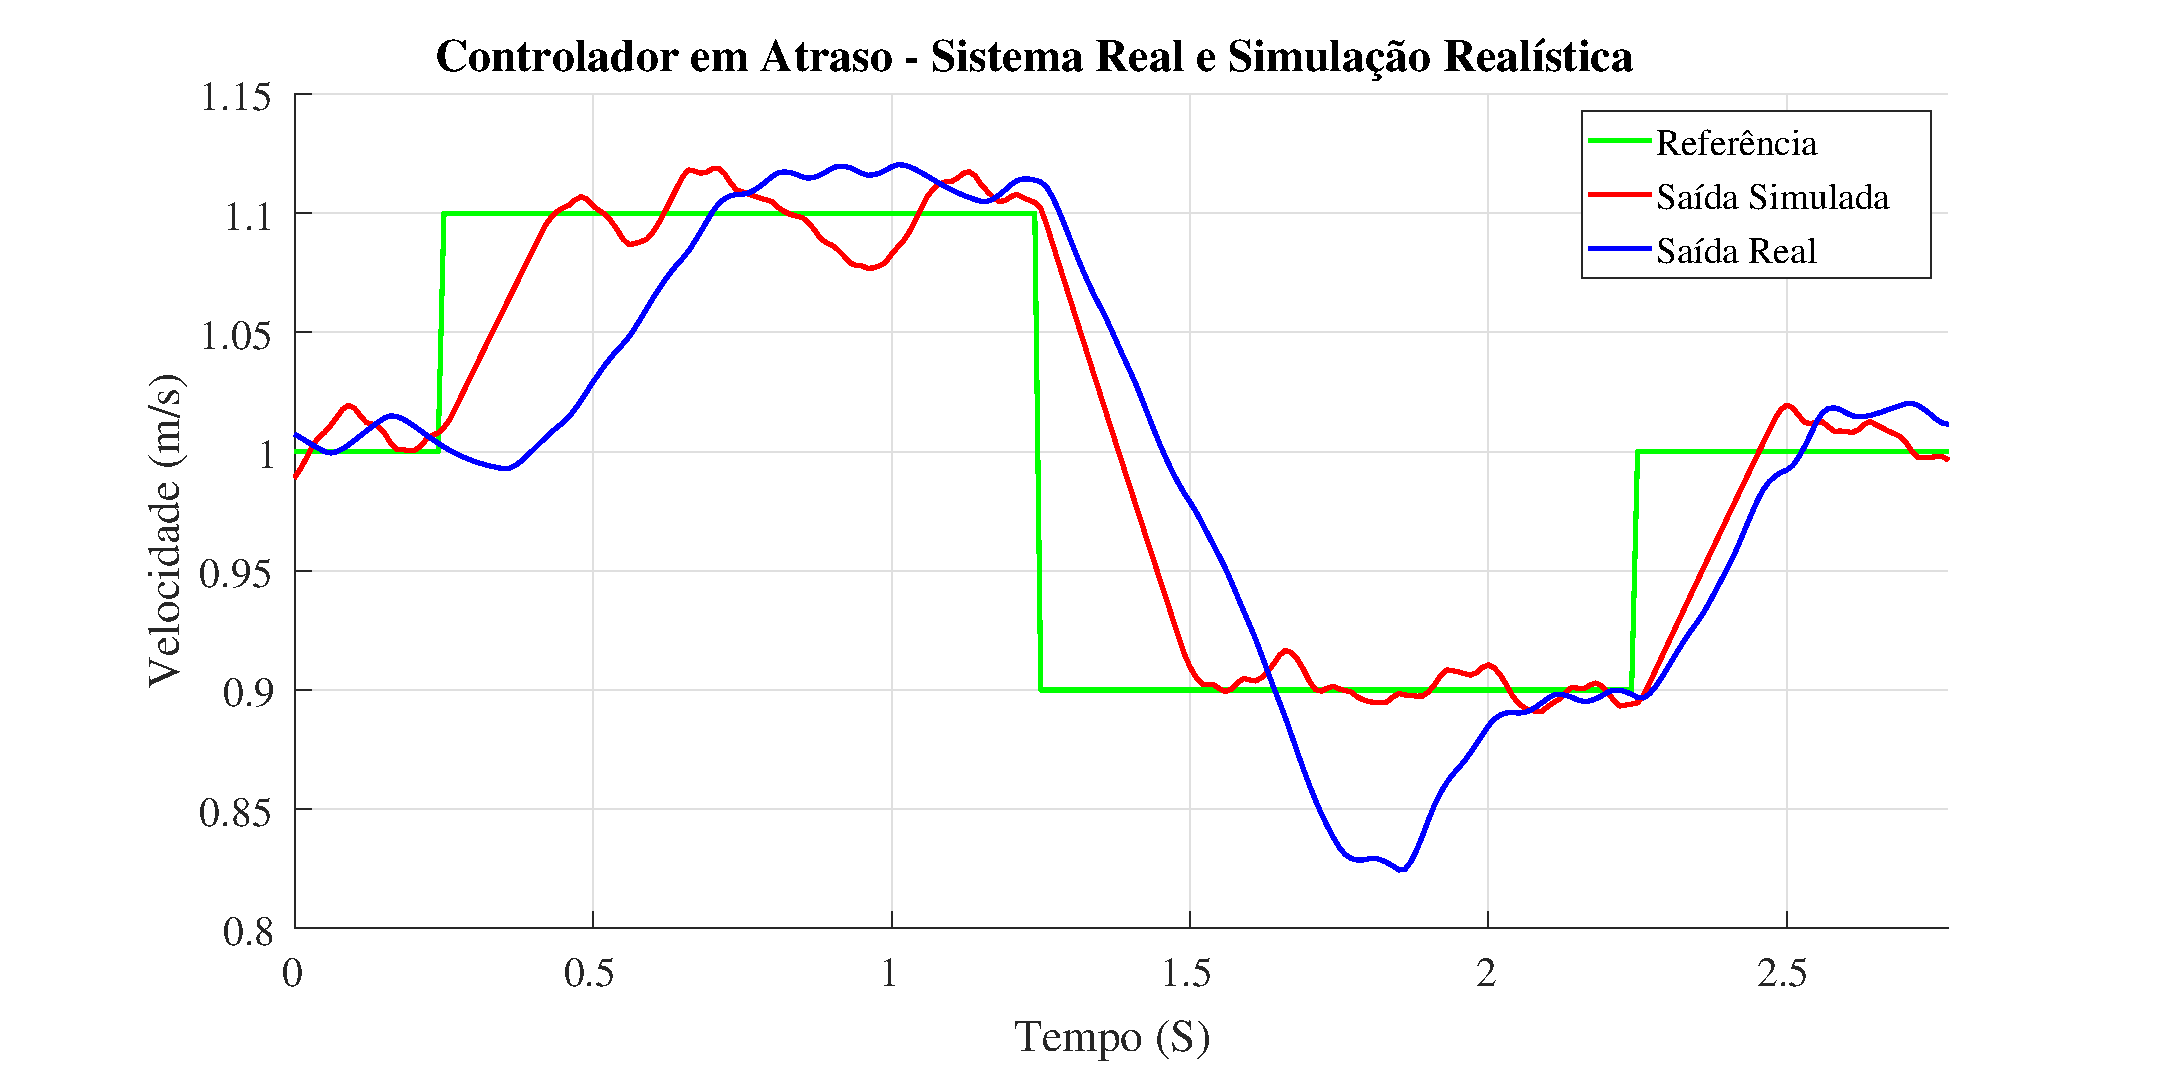
\includegraphics[width=0.5\textwidth]{imagens/atraso/compRealRealistica.eps}
                \caption{Comparação entre a saída do sistema real e a saída da simulação realística, com controlador em atraso de fase.}
                \label{fig:realistica_poli}
            \end{figure}
            
            Em comparação com a saída em simulação realística, o sistema apresenta dinâmicas similares, mas com variações referentes as perturbações encontradas e ruídos de leitura.
            
            Todos os resultados acima  tem ação \texttt{anti-windup} implementada. No gráfico abaixo é demonstrada o resultado do compensador em atraso com ação \texttt{anti-windup} ligada e desligada na planta real.
            
            \begin{figure}[H]
                \centering
                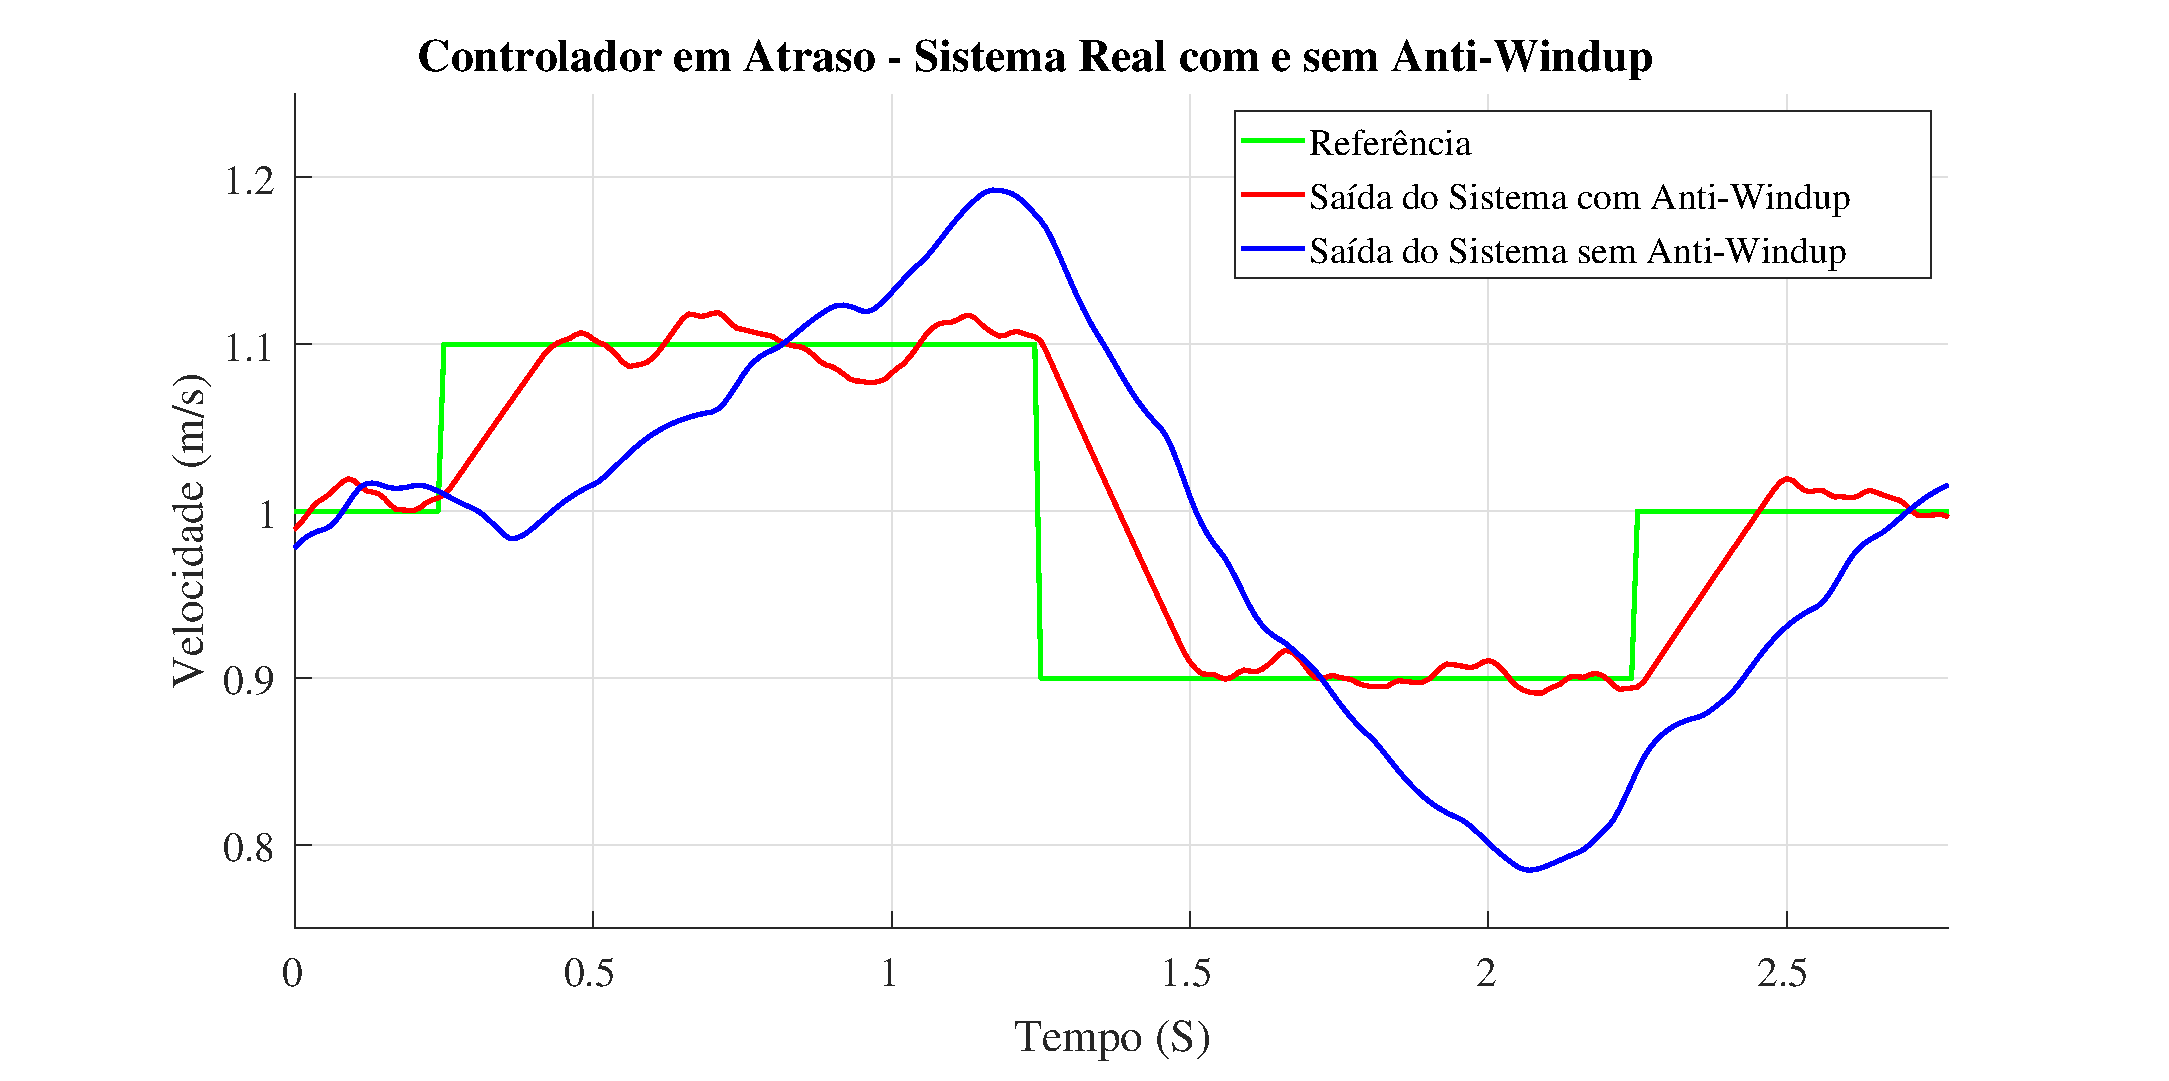
\includegraphics[width=0.5\textwidth]{imagens/atraso/compAntiWindup.eps}
                \caption{Comparação entre a resposta do sistema real com ação anti-windup e sem anti-windup.}
                \label{fig:realistica_poli_antiwindup}
            \end{figure}
            
            Como pode ser observado o sistema varia muito em torno da referência, a maior parte dos picos acentuados se deve que o sistema não descarrega o integrador assim que a saída cruza a referência, quando o mesmo é carregado pela saturação do controlador, o que torna o sistema menos confiável e mais instável.
        
    \section{Considerações Finais e Propostas Futuras}
    
    
    Os sistemas em malha fechada apresentaram desempenho bastante satisfatório em relação aos critérios definidos, tendo ambos respostas similares, mesmo com diferentes abordagens. A velocidade do veículo se tornou bastante estável. O sistema feito através do atraso de fase apresenta uma complexidade maior por ter um integrador, que acaba por vezes sobrecarregado pela saturação do sinald e controle, indicando a necessidade da implementação do sistema \texttt{anti-windup}.
    
    Mesmo com um sensor de má qualidade o sistema atendeu bem os critérios de desemprenho estabelecidos. A velocidade de leitura do sensor é extremamente ruidosa, variando com a taxa de amostragem. Diferente técnicas de filtragem de sinal foram aplicadas, com o fim de melhorar a visualização da velocidade real.
    
    Como proposta futura, com o desenvolvimento do controle mais preciso da velocidade, objetiva-se o equilíbrio do modelo de forma autônoma, o que era impossibilitado considerando que a velocidade do mesmo era inconstante.
    Trabalhar com a teoria e prática de um pêndulo invertido, que é um sistema de natureza instável, aplicando técnicas de controle afim de que o veículo se torne independente e consiga se equilibrar em condições normais de uso.
    
    
    \bibliography{referencias.bib}
    
\end{document}